\documentclass[a4paper]{article}
\usepackage[italian]{babel}
\usepackage[utf8]{inputenc}
\usepackage[T1]{fontenc}
\usepackage{graphicx}
\usepackage[export]{adjustbox}
\graphicspath{{./images/}{../cose da aggiungere/pittogrammi/}{../cose da aggiungere/privacy_conformita/}}
\usepackage{amsmath}
\usepackage{amsfonts}
\usepackage{amssymb}
\usepackage[version=4]{mhchem}
\usepackage{stmaryrd}

\usepackage{float}
\usepackage{tikz}
\usepackage{geometry}

\usepackage{titling}
\pretitle{\begin{center}
\includegraphics[width=\textwidth]{../cose da aggiungere/header_WATT+}\\[6em]}
	\posttitle{\end{center}}  

%\DeclareUnicodeCharacter{2713}{\ifmmode\checkmark\else{$\checkmark$}\fi}

\title{\Huge{BEAUTY BRIDGE}}
\date{}

\begin{document}
	
\maketitle

\begin{figure}[H]
	\centering
	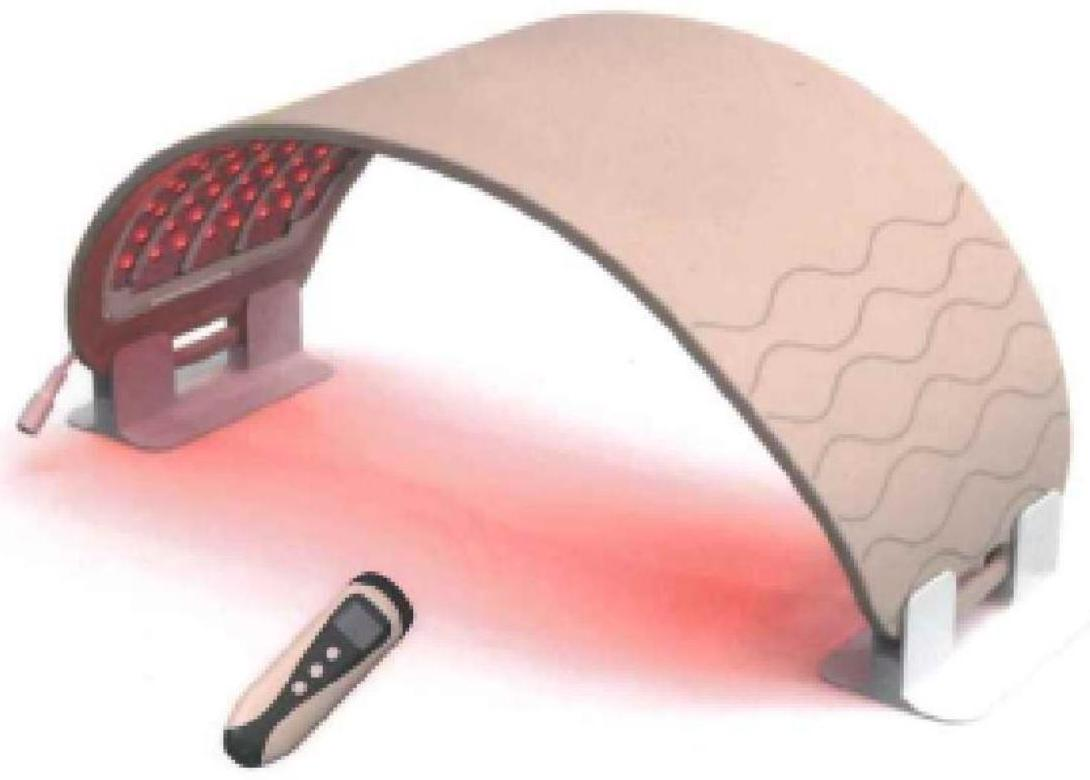
\includegraphics[width=0.8\textwidth]{15e924e1-b025-4d84-bbdd-92cf72f5ad6e-1_780_1090_1311_517}
%	\caption{}
\end{figure}

\newpage

\tableofcontents

\newpage

\section{ISTRUZIONI}
\begin{itemize}
	\item Schiarimento della pelle
	\item Azione rigenerativa
	\item Rimozione delle lenti, macchie e rughe.
	\item Tonificazione della pelle
	\item Trattamento dell'acne e sollievo dal dolore.
	\item Regolazione della produzione di sebo
\end{itemize}

\section{AVVERTENZE GENERALI}
Grazie per aver scelto il nostro dispositivo di fotobiostimolazione a LED. Leggere attentamente questo manuale prima dell'uso e seguire le avvertenze per garantire un utilizzo corretto e sicuro del prodotto.

Conservare questo manuale per eventuali riferimenti futuri.

\section{SIMBOLI}
\begin{figure}[H]
	\centering
	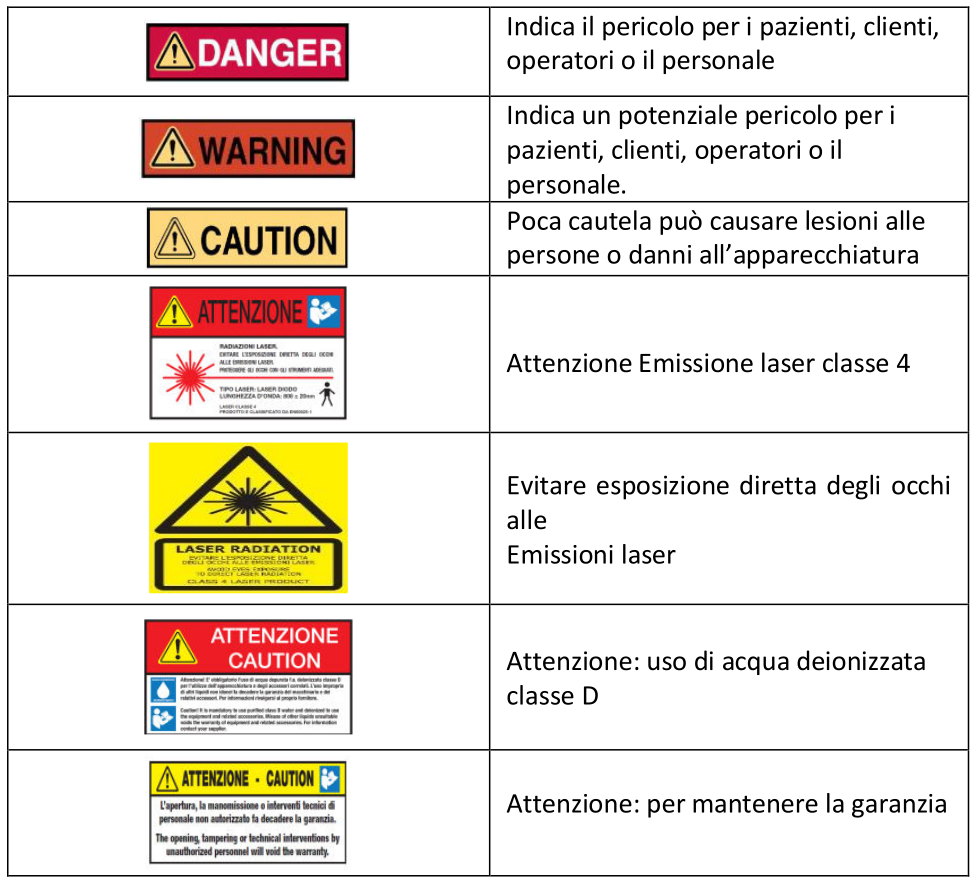
\includegraphics[width=\linewidth]{pittogrammi_1}
%	\caption{}
	\label{fig:pittogrammi1}
\end{figure}
\begin{figure}[H]
	\centering
	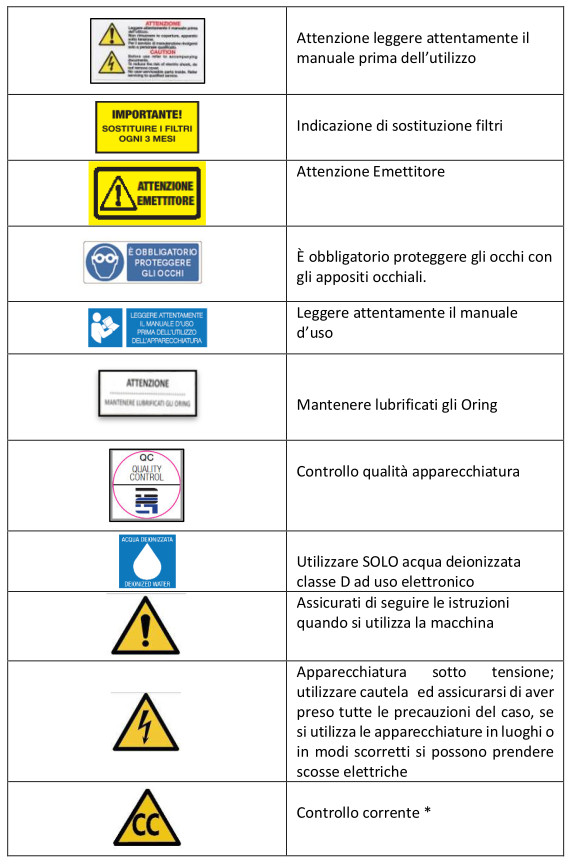
\includegraphics[width=\linewidth]{pittogrammi_2}
%	\caption{}
	\label{fig:pittogrammi2}
\end{figure}
\begin{figure}[H]
	\centering
	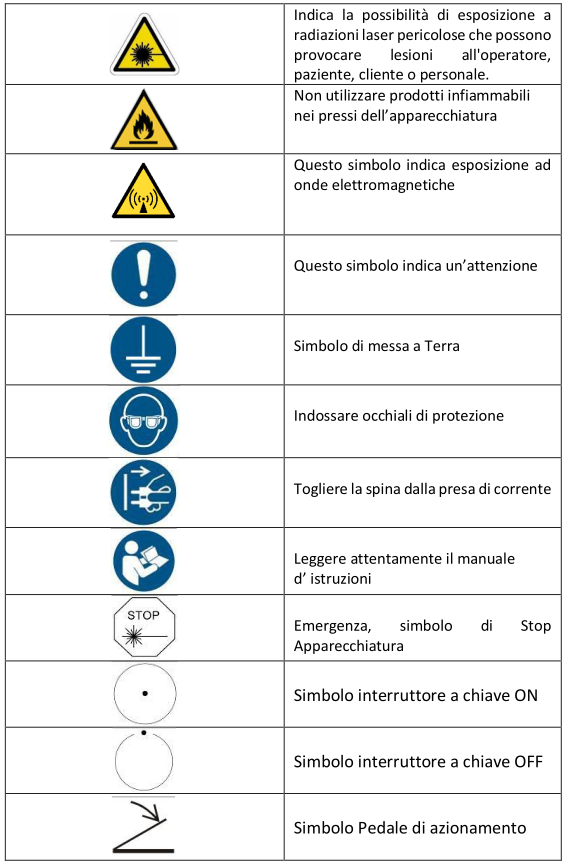
\includegraphics[width=\linewidth]{pittogrammi_3}
%	\caption{}
	\label{fig:pittogrammi3}
\end{figure}
\begin{figure}[H]
	\centering
	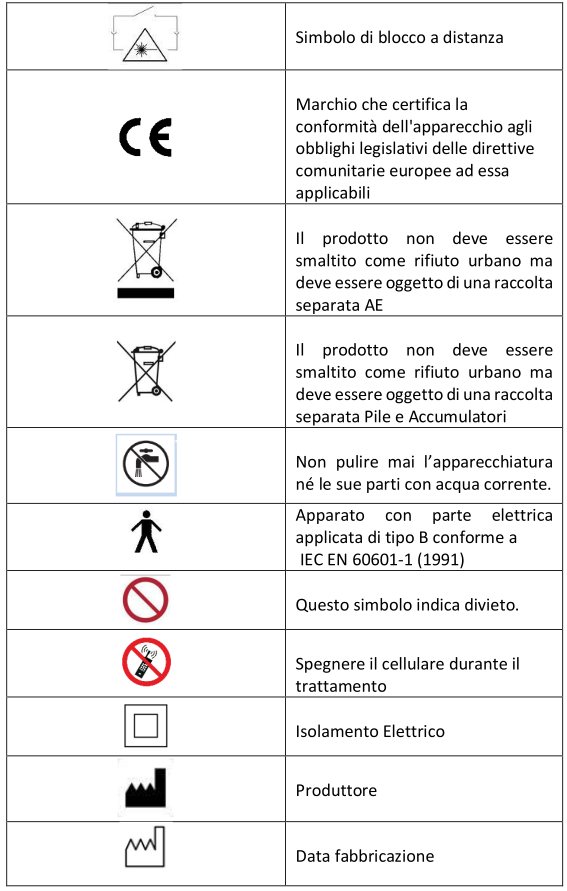
\includegraphics[width=\linewidth]{pittogrammi_4}
%	\caption{}
	\label{fig:pittogrammi4}
\end{figure}
\begin{figure}[H]
	\centering
	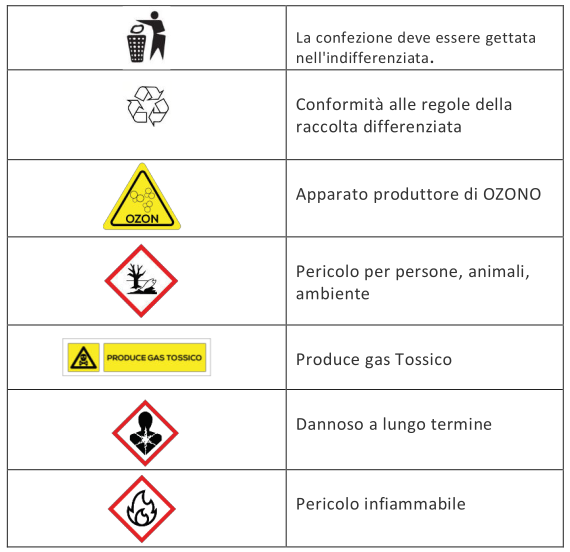
\includegraphics[width=\linewidth]{pittogrammi_5}
%	\caption{}
	\label{fig:pittogrammi5}
\end{figure}


\newpage

\section{PRINCIPIO DI FUNZIONAMENTO}
La World Medical Association (WMA) riconosce l'efficacia di specifiche onde luminose nell'attivazione dei processi di rigenerazione cellulare e tissutale.

Il dispositivo utilizza la fotobiostimolazione e la nanotecnologia per generare calore controllato e trasferire energia a bassa intensità e ad alta purezza. Questo favorisce la stimolazione dell'attività cellulare, con effetti naturali, sicuri e senza effetti collaterali, rendendolo adatto a tutti i tipi di pelle.

La radiazione luminosa viene assorbita dagli strati più profondi della pelle, dove l'energia viene convertita in energia intracellulare. Questo processo rilassa e rafforza i capillari, stimola le reazioni enzimatiche fotochimiche e aumenta l'attività della catalasi e della superossido dismutasi (SOD), che promuovono la degradazione dell'ATP, la principale fonte di energia cellulare.

Il risultato è un aumento del metabolismo e della sintesi cellulare, una maggiore produzione di collagene, una riorganizzazione delle fibre elastiche e del collagene e l'eliminazione della melanogenesi. Viene inoltre favorita la microcircolazione e stimolata la rigenerazione del tessuto connettivo.

\section{CARATTERISTICHE DEL DISPOSITIVO}
Il dispositivo portatile accelera la microcircolazione, migliora l'elasticità della pelle, combatte l'opacità e la illumina.

Integra 3 sorgenti LED con luce NIR con diverse onde luminose (blu, gialla, rossa) e una modalità FIR (infrarossi) specifica per vari problemi della pelle.

Luce blu + NIR(415 nm): Azione antibatterica e antinfiammatoria, utile contro acne, infiammazioni e lesioni cutanee. Favorisce una guarigione ottimale e una migliore rigenerazione.

Luce gialla + NIR(590 nm): stimola il metabolismo cellulare, favorisce il drenaggio linfatico, riduce la pigmentazione e il rossore, tratta il rossore e migliora l'immunità della pelle.

Luce rossa + NIR(630 nm): Riattiva l'attività cellulare, accelera la sintesi del collagene, ha un effetto anti-invecchiamento, schiarente, tonificante e antiossidante.

Luce infrarossa (FIR)(850 nm): Migliora la circolazione sanguigna e l'ossigenazione dei tessuti, favorisce la riparazione dei tessuti, riduce il dolore muscolare e articolare.

\section{ATTREZZATURA}
\begin{itemize}
	\item $1 \times$ dispositivo principale in silicone PDT
	\item $1 \times$ Telecomando
	\item $1 \times$ cavo di ricarica USB
	\item 1 adattatore $12 \mathrm{~V} / 4 \mathrm{~A}$
	\item $1 \times$ Poggiatesta
\end{itemize}

\begin{figure}[H]
	\centering
	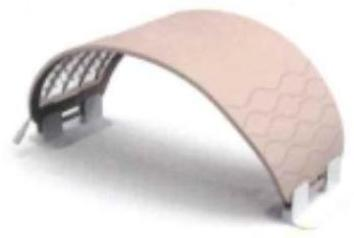
\includegraphics[width=0.7\textwidth]{15e924e1-b025-4d84-bbdd-92cf72f5ad6e-3_238_354_1271_1069}
%	\caption{}
\end{figure}

\begin{figure}[H]
	\centering
	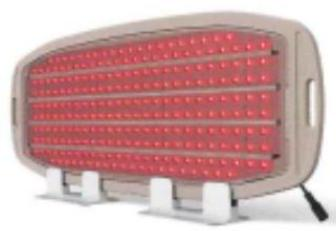
\includegraphics[width=0.7\textwidth]{15e924e1-b025-4d84-bbdd-92cf72f5ad6e-3_231_336_1280_1544}
%	\caption{}
\end{figure}

\begin{itemize}
	\item $1 \times$ Cinghia di fissaggio
	\item $1 \times$ Occhiali protettivi
	\item $2 \times$ Staffe di supporto
	\item $1 \times$ Manuale utente
\end{itemize}
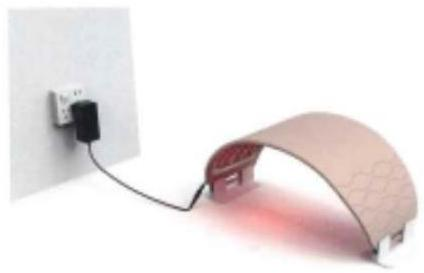
\includegraphics[max width=\textwidth, alt={}, center]{15e924e1-b025-4d84-bbdd-92cf72f5ad6e-3_273_424_1607_1031}\\
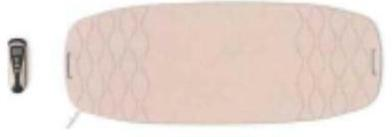
\includegraphics[max width=\textwidth, alt={}, center]{15e924e1-b025-4d84-bbdd-92cf72f5ad6e-3_137_392_1718_1521}

\section{ISTRUZIONI PER L'USO}
Pulire accuratamente la pelle e asciugarla con un panno morbido.\\
Collegare il dispositivo al controller tramite il cavo USB.

Accedere al dispositivo prima di premere il pulsante di accensione.\\
Selezionare la modalità luminosa con il colore del gusto, l'intensità (50,75,100\%) e impostare il tempo di elaborazione desiderato (si consigliano 15-30 minuti). Non guardare direttamente la fonte di luce.

Posizionare il cinturino attraverso i fori corrispondenti alle estremità del dispositivo. Modellare il dispositivo in un Utilizzare l'arco per adattarlo al viso o applicarlo al corpo o alle gambe. Si consiglia di utilizzarlo in posizione supina. per favorire il rilassamento.

Dopo aver completato il trattamento, attivare il dispositivo e pulirlo accuratamente.

\section{PRECAUZIONI PER L'USO}
Non guardare direttamente la fonte di luce. Tenere gli occhi chiusi durante l'uso e proteggerli con occhiali di sicurezza adeguati.

Evitare di forare o danneggiare la superficie del LED.\\
Non immergere il dispositivo in acqua. Pulirlo con un panno umido.\\
Non utilizzare solventi chimici aggressivi.\\
Evitare l'esposizione diretta alla luce solare.\\
Pulire accuratamente il dispositivo dopo l'uso.

\section{CONTROINDICAZIONI}
Non usare in caso di gravidanza, epilessia, malattie della tiroide, allergie fotosensibili o terapie farmacologiche fotosensibilizzanti, lesioni cutanee o traumi.

Non usare sui bambini.\\
In caso di eventi avversi o incidenti, interrompere l'uso e consultare un medico.

\section{ASSISTENZA E GARANZIA}
Garanzia di 12 mesi dalla data di acquisto (non copre i danni dovuti a usura o uso improprio).\\
Conservare la ricevuta e il sigillo del rivenditore per eventuali interventi in garanzia.\\
L'adattatore e il cavo dati non sono coperti dalla garanzia per la normale usura.\\
La garanzia è valida per dieci anni in caso di manomissione o riparazioni non autorizzate.\\
Le spese di spedizione sono a carico dell'utente.

Per assistenza, contattare il distributore o il produttore.

\section{SPECIFICHE TECNICHE}
\begin{itemize}
	\item Modello: G240
	\item Potenza nominale: 40 W
	\item Numero di LED: 960
	\item Modalità LED: 5050
	\item Rapporto LED: 415:590:630:850 = 1:1:1:1
	\item Dimensioni: $680 \times 257 \times 8,5 \mathrm{~mm}$
	\item Peso: 1.300 g (compreso il controller)
	\item Regolazione: 4 modalità, 3 livelli di luminosità, timer.
	\item Regolatore del tempo di ricarica: 2,5 minerali
\end{itemize}

\section{DESCRIZIONE DEI PULSANTI DEL CONTROLLER}
\begin{itemize}
	\item Mostra il livello di potenza
	\item Orario dello spettacolo
	\item Modalità di visualizzazione
	\item Visualizzazione del segnale di connessione
	\item Luminosità dello schermo
	\item Pulsante di accensione/modalità
	\item Timer del sapore
	\item Pulsante luminosità
	\item Porta di ricarica di tipo C
\end{itemize}

\begin{figure}[H]
	\centering
	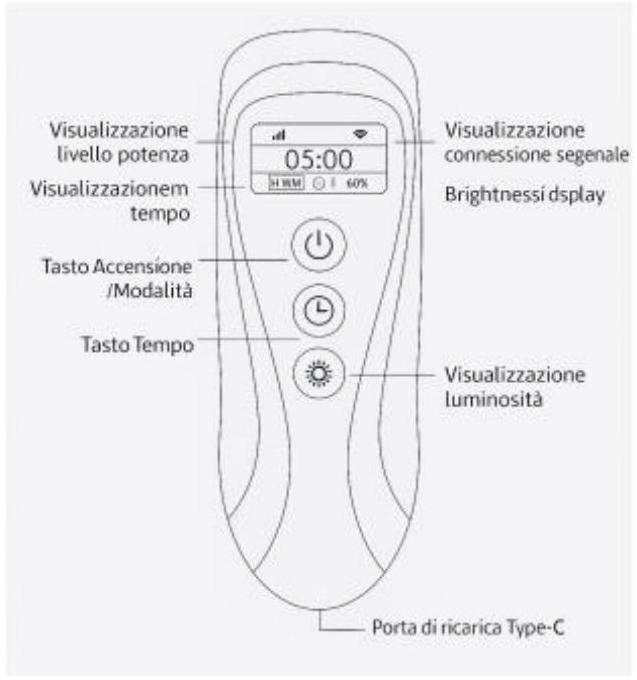
\includegraphics[width=0.7\textwidth]{15e924e1-b025-4d84-bbdd-92cf72f5ad6e-5_680_637_1398_1342}
%	\caption{}
\end{figure}

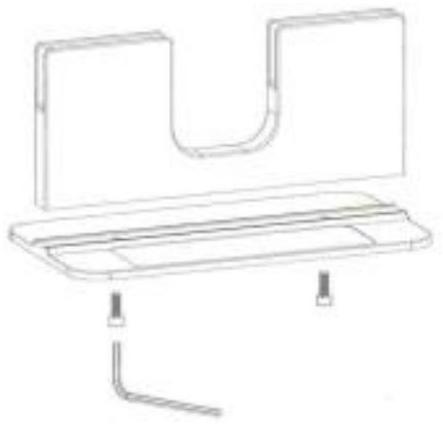
\includegraphics[max width=\textwidth, alt={}, center]{15e924e1-b025-4d84-bbdd-92cf72f5ad6e-5_424_443_2277_524}\\
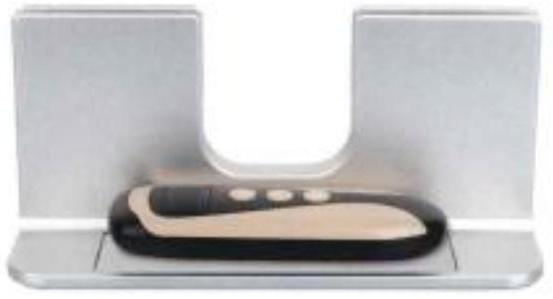
\includegraphics[max width=\textwidth, alt={}, center]{15e924e1-b025-4d84-bbdd-92cf72f5ad6e-5_299_553_2320_1082}


\newpage

\section{CONSENSO INFORMATO - Trattamento estetico "BEAUTY BRIDGE+"}
\subsection{DATI CLIENTE}
Nome e Cognome: $\_\_\_\_$\\
Data di nascita: $\_\_\_\_$\\
Telefono: $\_\_\_\_$

\subsection{DATI OPERATORE / CENTRO}
Nome centro: $\_\_\_\_$\\
Operatore: $\_\_\_\_$

\subsection{DESCRIZIONE DEL TRATTAMENTO}
Il trattamento Beauty Bridge+ utilizza una tecnologia combinata a infrarossi e cromoterapia applicata tramite ponte facciale, finalizzata a stimolare la microcircolazione, migliorare la tonicità cutanea e favorire il benessere della pelle.

\subsection{POSSIBILI EFFETTI}
Lieve arrossamento temporaneo, sensazione di calore, lieve sensibilità cutanea.

\subsection{CONTROINDICAZIONI}
Gravidanza, patologie cutanee attive, fotosensibilità, problemi circolatori importanti, patologie oncologiche in corso, infezioni o infiammazioni nella zona trattata.

\subsection{DICHIARAZIONI DEL CLIENTE}
Dichiaro di aver ricevuto spiegazioni chiare, di essere a conoscenza che si tratta di trattamento estetico e non medico, e di autorizzare l'esecuzione del trattamento.

\subsection{PRIVACY}
I dati saranno trattati nel rispetto del Regolamento UE 2016/679 (GDPR).\\
Firma Cliente: $\_\_\_\_$\\
Firma Operatore: $\_\_\_\_$\\
Data: $\_\_\_\_$ / $\_\_\_\_$ / $\_\_\_\_$


% --- INIZIO INFORMATIVA PRIVACY ---
\newpage

\section{INFORMATIVA PRIVACY}
\begin{center}
	(ai sensi dell'art. 13 del Regolamento UE 2016/679)
\end{center}

La presente informativa è resa ai sensi del Regolamento Generale sulla Protezione dei Dati (GDPR) e riguarda il trattamento dei dati personali dei clienti che si sottopongono a trattamenti e tecnologie estetiche.

\subsection*{Titolare del trattamento}

Il Titolare del trattamento è:

\begin{itemize}
	\item Denominazione centro estetico: \underline{\hspace{5cm}}
	\item Sede legale: \underline{\hspace{7cm}}
	\item P. IVA / C.F.: \underline{\hspace{6cm}}
	\item Contatti (telefono/email): \underline{\hspace{5cm}}
\end{itemize}

\subsection*{Tipologia di dati trattati}

Il Titolare può raccogliere e trattare le seguenti categorie di dati:

\begin{itemize}
	\item Dati anagrafici (nome, cognome, data di nascita)
	\item Dati di contatto (telefono, e-mail)
	\item Dati fiscali per eventuale fatturazione
	\item Dati particolari relativi allo stato di salute (allergie, patologie, gravidanza, terapie in corso) necessari per valutare l'idoneità ai trattamenti estetici
	\item Eventuali immagini fotografiche prima/dopo trattamento (previo consenso specifico)
\end{itemize}

\subsection*{Finalità del trattamento}

I dati personali sono trattati per le seguenti finalità:

\begin{enumerate}
	\item Esecuzione di trattamenti estetici e utilizzo di tecnologie professionali (laser, radiofrequenza, ultrasuoni, pressoterapia, ecc.)
	\item Valutazione dell'idoneità al trattamento
	\item Adempimenti amministrativi, contabili e fiscali
	\item Gestione degli appuntamenti
	\item Eventuale invio di comunicazioni promozionali (solo previo consenso separato)
	\item Eventuale utilizzo di immagini per finalità informative o promozionali (solo previo consenso separato)
\end{enumerate}

\subsection*{Base giuridica del trattamento}

Il trattamento dei dati si fonda su:

\begin{itemize}
	\item Esecuzione del contratto/prestazione richiesta
	\item Adempimento di obblighi di legge
	\item Consenso esplicito dell'interessato per il trattamento di dati particolari (sanitari)
	\item Consenso separato per marketing e utilizzo immagini
\end{itemize}

\subsection*{Modalità di trattamento}

Il trattamento dei dati avviene mediante strumenti cartacei e/o informatici, nel rispetto dei principi di correttezza, liceità, trasparenza e tutela della riservatezza.

Sono adottate adeguate misure di sicurezza per prevenire accessi non autorizzati, perdita o diffusione dei dati.

\subsection*{Conservazione dei dati}

I dati personali saranno conservati:

\begin{itemize}
	\item Per il tempo necessario all'erogazione del servizio
	\item Per il periodo previsto dalla normativa fiscale e civilistica
	\item Fino a revoca del consenso per finalità di marketing o utilizzo immagini
\end{itemize}

\subsection*{Comunicazione dei dati}

I dati potranno essere comunicati a:

\begin{itemize}
	\item Consulenti fiscali e amministrativi
	\item Software gestionali utilizzati per la gestione clienti
	\item Autorità competenti, ove previsto dalla legge
\end{itemize}

I dati non saranno diffusi senza consenso.

\subsection*{Diritti dell'interessato}

L'interessato può esercitare in qualsiasi momento i seguenti diritti:

\begin{itemize}
	\item Accesso ai propri dati
	\item Rettifica o aggiornamento
	\item Cancellazione (diritto all'oblio)
	\item Limitazione del trattamento
	\item Opposizione al trattamento
	\item Revoca del consenso
	\item Reclamo all'Autorità Garante per la Protezione dei Dati Personali
\end{itemize}

Le richieste possono essere inviate ai recapiti del Titolare sopra indicati.

\subsection*{Natura del conferimento dei dati}

Il conferimento dei dati è necessario per l'erogazione dei trattamenti estetici.
Il mancato conferimento può comportare l'impossibilità di eseguire il servizio.

\subsection*{CONSENSO}

Il/La sottoscritto/a dichiara di aver ricevuto e compreso la presente informativa.

\vspace{0.8cm}

Data: \underline{\hspace{5cm}} 

\vspace{15pt}
Firma: \underline{\hspace{6cm}}

\vspace{1cm}

$\square$ Acconsento al trattamento dei dati particolari (sanitari)

\vspace{0.3cm}
$\square$ Acconsento all'utilizzo delle immagini per finalità promozionali

\vspace{0.3cm}
$\square$ Acconsento a ricevere comunicazioni promozionali

% --- FINE INFORMATIVA PRIVACY ---

\newpage


\begin{figure}[H]
	\centering
	\includegraphics[width=0.7\paperwidth,height=\paperheight, keepaspectratio]{"../cose da aggiungere/privacy_conformita/dichiarazione_conformita"}
\end{figure}





\end{document}